\documentclass{sigchi}
% Use this command to override the default ACM copyright statement (e.g. for preprints). 
% Consult the conference website for the camera-ready copyright statement.


%% EXAMPLE BEGIN -- HOW TO OVERRIDE THE DEFAULT COPYRIGHT STRIP -- (July 22, 2013 - Paul Baumann)
% \toappear{Permission to make digital or hard copies of all or part of this work for personal or classroom use is 	granted without fee provided that copies are not made or distributed for profit or commercial advantage and that copies bear this notice and the full citation on the first page. Copyrights for components of this work owned by others than ACM must be honored. Abstracting with credit is permitted. To copy otherwise, or republish, to post on servers or to redistribute to lists, requires prior specific permission and/or a fee. Request permissions from permissions@acm.org. \\
% {\emph{CHI'14}}, April 26--May 1, 2014, Toronto, Canada. \\
% Copyright \copyright~2014 ACM ISBN/14/04...\$15.00. \\
% DOI string from ACM form confirmation}
%% EXAMPLE END -- HOW TO OVERRIDE THE DEFAULT COPYRIGHT STRIP -- (July 22, 2013 - Paul Baumann)


% Arabic page numbers for submission. 
% Remove this line to eliminate page numbers for the camera ready copy
\pagenumbering{arabic}


% Load basic packages
\usepackage{balance}  % to better equalize the last page
\usepackage{graphics} % for EPS, load graphicx instead
\usepackage{times}    % comment if you want LaTeX's default font
\usepackage{url}      % llt: nicely formatted URLs
\usepackage{verbatim}
\usepackage{tabularx}
% llt: Define a global style for URLs, rather that the default one
\makeatletter
\def\url@leostyle{%
  \@ifundefined{selectfont}{\def\UrlFont{\sf}}{\def\UrlFont{\small\bf\ttfamily}}}
\makeatother
\urlstyle{leo}


% To make various LaTeX processors do the right thing with page size.
\def\pprw{8.5in}
\def\pprh{11in}
\special{papersize=\pprw,\pprh}
\setlength{\paperwidth}{\pprw}
\setlength{\paperheight}{\pprh}
\setlength{\pdfpagewidth}{\pprw}
\setlength{\pdfpageheight}{\pprh}

% Make sure hyperref comes last of your loaded packages, 
% to give it a fighting chance of not being over-written, 
% since its job is to redefine many LaTeX commands.
\usepackage[pdftex]{hyperref}
\hypersetup{
pdftitle={SIGCHI Conference Proceedings Format},
pdfauthor={LaTeX},
pdfkeywords={SIGCHI, proceedings, archival format},
bookmarksnumbered,
pdfstartview={FitH},
colorlinks,
citecolor=black,
filecolor=black,
linkcolor=black,
urlcolor=black,
breaklinks=true,
}

% create a shortcut to typeset table headings
\newcommand\tabhead[1]{\small\textbf{#1}}


% End of preamble. Here it comes the document.
\begin{document}

\title{Voice Interfaces for Visually Impaired and Low-Literate Communities in the Developing World}

\numberofauthors{2}
\author{
  \alignauthor Aditya Vashistha\\
    \email{adityav@cs.washington.edu}\\
   \alignauthor Sam Sudar\\
    \email{sudars@cs.washington.edu}\\}

\maketitle

\begin{abstract}
Millions of people cannot access services using conventional graphical user interfaces. These users include the visually impaired, the low-literate, speakers of tribal languages without font support, and those without access to computers or mobile devices. Interactive voice response (IVR) systems provide a way to interact with users without the need for graphics. Callers are read options and use the keypad to navigate the content, lowering the barriers for access and providing the opportunity for engagement. Current IVR systems provide a wide spectrum of services, including health information, citizen journalism, and social media. However, little work has been done to inform the organization of IVR content. We compare list, shallow and deepr hierarchies to organize content in an IVR system, expanding on similar work that has focused on graphical user interfaces. We find that both flat lists and deep hierarchies are inappropriate, and that shallow hierarchies create a more effective IVR structure.
\end{abstract}


\begin{comment}


\keywords{
	Guides; instructions; author's kit; conference publications;
	keywords should be separated by a semi-colon.
	\textcolor{red}{Mandatory section to be included in your final version.}
}

\category{H.5.m.}{Information Interfaces and Presentation (e.g. HCI)}{Miscellaneous}

See: \url{http://www.acm.org/about/class/1998/}
for more information and the full list of ACM classifiers
and descriptors. 
\textcolor{red}{Mandatory section to be included in your
final version. On the submission page only the classifiers'
letter-number combination will need to be entered.}

\end{comment}

\section{Introduction}
According to the World Health Organization, 285 Million people in the world are visually impaired (VI) and 90\% of them live in developing countries \cite{WHO2013}. VI people in developing countries have limited access to assistive technologies because of various socio-economic, device-related and network related constraints. In India, only
5\% of all mobile phone subscribers own a smartphone \cite{Mary2013}. The remaining 95\% use a basic or feature phone; these typically have only one inbuilt assistive tool for VI people: a speaking clock. Lack of screen readers on these devices and tactile interfaces force VI users to access information and provide data using voice based communication on their phones. 

The literacy rate in most developing countries is quite low. For example, 26\% people in India are illiterate and the rate of functional illiteracy is surprisingly high. Even in a developed country like US where the claimed literacy rate is 99\%, around 20\% of adults are functionally illiterate. Thus, text based interfaces are out of reach of sighted low-literate communities as well. In India, there are millions of speakers of tribal languages like Kui, Kurukh, Gondi. However, the font support for many tribal languages is still non-existent. Thus many literate tribal people also use voice medium for producing and accessing information. The limited usage of computing devices like smartphones, tablets, and desktops limits adoption of graphical user interfaces designed for low-literate low-income communities. As a result, these communities also use their basic or feature phones to access informational services on the voice channel.

In recent years, various researchers and practitioners have used Interactive Voice Response (IVR) systems to provide health information, citizen journalism, educational services, feedback channels, data collection systems, social media platform, etc. for low-literate marginalized communities. IVR systems have also been used as a means to provide information to and collect data from VI people with low socio-economic status. Though there are a lot of success stories of organizations appropriating IVR systems for societal development, there are a number of challenges that impede the sustainable usage of such systems. The first challenge is the high cost of calls for accessing information. The second challenge is inefficient audio content management. Hierarchical call trees are used in IVR systems to structure the information much like a menu in graphical user interfaces. However, auditory interfaces are quite different from textual and graphical interfaces. Voice interfaces force users to access information sequentially, which results in frustration, high cost, and low-usability. Moreover, searching and indexing audio recordings on an IVR system are non-trivial operations because of unavailability of high efficacy speech recognition engines for resource constrained languages spoken in developing countries. Because of the above reasons, concentrated efforts are needed for accurate and swift retrieval of information to decrease the time required by callers and to increase usability. 

Our aim is to understand ways in which voice interfaces on an IVR platform can be organized so as to optimize information seeking time, information absorption, and call duration. Through this project, we are evaluating expressiveness and effectiveness of various voice interface designs for providing information to low-literate and VI communities. Our research will answer the following research questions:

\begin{itemize}
\item Is a hierarchical voice menu better than a linear list?
\item How many items are acceptable in a linear list?
\item Is a shallow hierarchy better than deep hierarchy?
\item How deep or shallow the hierarchy should be?
\item How do abstraction capabilities, literacy level, and prior exposure to IVR impact different designs of voice user interfaces? 
\end{itemize}


\section{Related Work}

\subsection{Interfaces for Low-Literate People}
A lot of work has been done in designing user interfaces for low-literate low-income communities in the developing world. Most of the work explores usage of graphical interfaces \cite{Grisedale1997,Medhi2011a,Medhi2008,Ghosh2003} and auditory interfaces \cite{Cuendet2013,Agarwal2010,Mudliar2013} for collecting data and providing information to marginalized low-literate communities. Various researchers have explored challenges faced by literate users while accessing hierarchical menus \cite{Allen1983,Chaudry2012}. However, the most relevant work to our project is done by Medhi et. al., where they presented how limited education affects hierarchical user interface navigation on desktops and mobile phones \cite{Medhi2013a,Medhi2013b}. Medhi measured the textual literacy level and abstract reasoning level for low-income low-literate people in India. The participants were then asked to find items from graphical user interfaces consisting of a linear list, shallow, and deep hierarchy. Medhi found that low-income, low-literate communities performed best when navigating a linear structure on both desktops as well as mobile phones.

\subsection{Interfaces for VI People}
Although VI people can use screen readers to access information on the Internet, this requires a computer/smartphone, expensive screen reader software, and an Internet connection that is beyond the reach of the majority of the low-income VI people in the developing world \cite{McCarthy2012}. Our parallel research (under review in MobileHCI 2014) has demonstrated that many low-income VI people do not use screen reader software, instead using alternative information and communication tools for accessing information. Many participants of the study indicated using IVR systems for accessing educational and entertainment content. Some work has also been done to augment or replace visual menus on desktops, mobile phones and other electronic devices like music players for improved usability and accessibility \cite{Yalla2008,Zhao2007,Jeon2012}. However, no work has yet been done to understand the trade-offs between using lists and different kind of hierarchical interfaces to organize information in IVR systems.

\subsection{IVR Design Guidelines}
Various researchers have provided design guidelines to create effective IVR systems and decrease cognitive load on callers	 \cite{Ndwe2008,Suhm2008,MSDNSpeech,Halstead-Nussloch1989}. However, few guidelines focus on the breadth and depth of navigation IVR trees. Various researchers have investigated deep and shallow hierarchies in IVR systems for high-literate users in the developed world \cite{Huguenard1997,Virzi1997,Commarford2008}. For instance, Commarford et.al. compared deep and shallow IVR hierarchies and concluded that deep hierarchies take longer to navigate and have high cognitive load \cite{Commarford2008}. However, the participants of the study were undergraduate students with at least three months of email experience and were based in the United States. 

Researchers have also studied various facets of IVR systems to improve information consumption and production by low-income low-literate populations in the developing world. Chakraborty et.al. has provided design guidelines for creating IVR surveys for low-literate low-income marginalized communities in India \cite{Chakraborty2013}. Kummamuru et.al. has analyzed the relationship between cognitive load and various navigational factors like breadth, depth, type of information, and numerical order \cite{Kummamuru2012}. They asked semi-literate participants in India to find job information from a synthetic IVR job repository. Each participant had to complete eight tasks. The tasks were designed such that the impact of depth, breadth and other parameters on cognitive load could be measured. They found that the time to choose the correct option decreases as the breadth and depth increases. This is because practice and learning effects impact the time taken to navigate the depth. Moreover, cognitive load is high while listening to the first few options in the breadth and thus the navigation time is lessened for later options in the breadth. The biggest weakness of the paper is the absence of direct comparisons between linear lists, shallow hierarchies and deep hierarchies.

To the best of our knowledge, our work will be the first to directly compare linear list, shallow hierarchy and deep hierarchy for maximizing information absorption by low-literate low-income communities and visually impaired people in India. 

\section{Design}
We have conducted three between-subjects experiments to compare three designs of IVR interfaces: linear list, shallow hierarchical interface, and deep hierarchical interface. We have used the \textit{Household items} dataset used by researchers for comparing performance of low-literate communities using these structures with graphical user interfaces \cite{Medhi2013a,Medhi2013b}. We chose the same dataset in order to directly compare our finding with the findings for graphical visualizations. In our experiment, each structure is read aloud by the system. The list user interface is a sequential list of the household items. The shallow hierarchical interface has a branching factor of five and the depth of the tree is two (see Figure 1). The branching factor for the deep hierarchical interface is up to four, and the depth of the tree is four (see Figure 2). We have implemented the design structures in VoiceXML using Voxeo Prophecy and IVR Junction \cite{Vashistha}. We logged users' interaction with the IVR system while performing tasks in order to review the actions users took while performing the tasks.

\begin{figure}[!h]
\centering
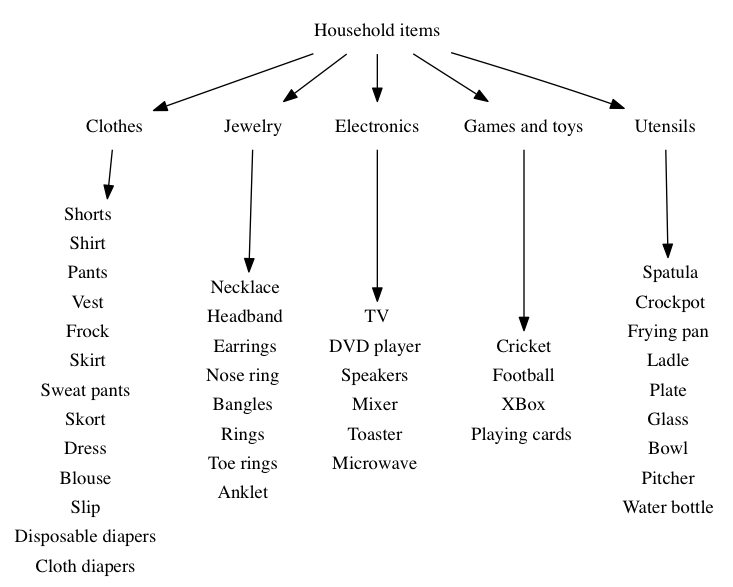
\includegraphics[width=0.9\columnwidth]{ShallowHierarchy}
\caption{Shallow hierarchy arrangement of household items}
\label{fig: Figure1}
\end{figure}

\begin{figure}[!h]
\centering
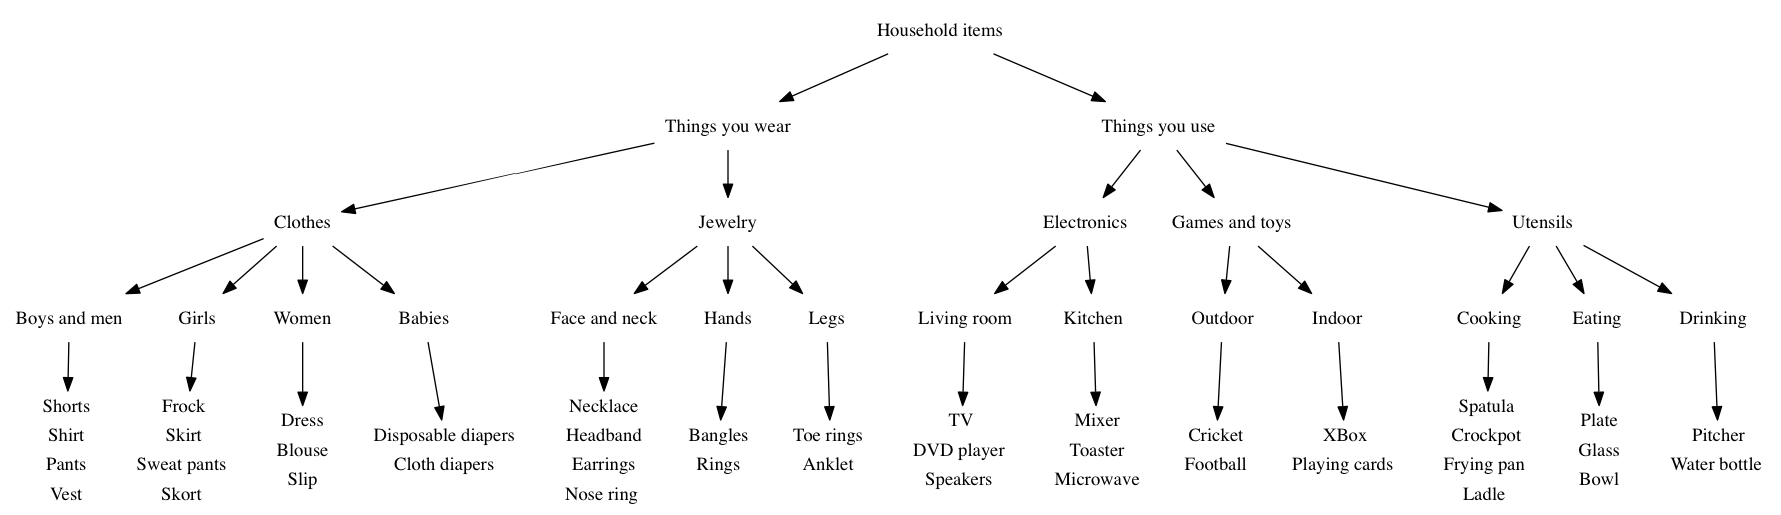
\includegraphics[width=0.9\columnwidth]{DeepHierarchy}
\caption{Deep hierarchy arrangement of household items}
\label{fig: Figure2}
\end{figure}

Participants were randomly divided into 3 groups where each group contained equal numbers of participants. Each participant performed five tasks, one after another. Each task consisted of selecting a target item from the assigned design structure. All participants searched for five target items (Shirt, Blouse, Rings, Football, and Plate) in the same order. We did not randomize the tasks for participants to ensure that the learning effects for each participant was the same. We selected two easy tasks (\textit{find Shirt, Blouse}), one task of intermediate difficulty (\textit{find Rings}), and two complex tasks (\textit{find Football, Plate}). The comparative complexity of performing a particular task (say \textit{find Rings}) across different hierarchies is defined as requiring the same number of hops to reach the target item (excluding navigational prompts) in a brute force manner.  

\section{Evaluation}
We recruited 18 participants (12 Male, 6 Female) to evaluate the three design structures. All the participants were either students or employees of the Computer Science and Engineering Department of the University of Washington. The average age of the participants was 26.7 years (max=52, min=19) and the average education level was Master's. Sixteen participants were heavy users and two were moderate users of IVR systems. None of the participants were visually impaired. 

Before beginning the experiment, participants were shown a demonstration task where they had to find an item from the randomly assigned design structure. We used a different dataset (animals) to illustrate the task and design structure to participants. Participants were allowed to perform demo task at most two times before starting the actual experimental task. We also observed participants while they were performing the task for understanding the challenges they faced while navigating design structures. After completing the task, we interviewed participants to collect demographic information. Participants also completed a short survey where they rated their performance, frustration, and physical, temporal and mental efforts exuded while performing the tasks. 

The following criteria were used for evaluating information absorption and swiftness in navigating the design structures:
\begin{itemize}
\item Task completion rate
\item Task correctness
\item Average task completion time
\end{itemize}

Correctness of a task is defined as whether or not the subject correctly selected the target item. For example, if the task was \textit{find Shirt} and the subject made any final selection other than \textit{Shirt}, it was defined as incorrect. The list structure resulted in the lowest correctness, with an overall correctness rate of 57\% across all the tasks. The shallow hierarchy achieved a 93\% correctness rate, while the deep hierarchy fared slightly better with 97\% accuracy rate.

\begin{figure}[!h]
    \centering
    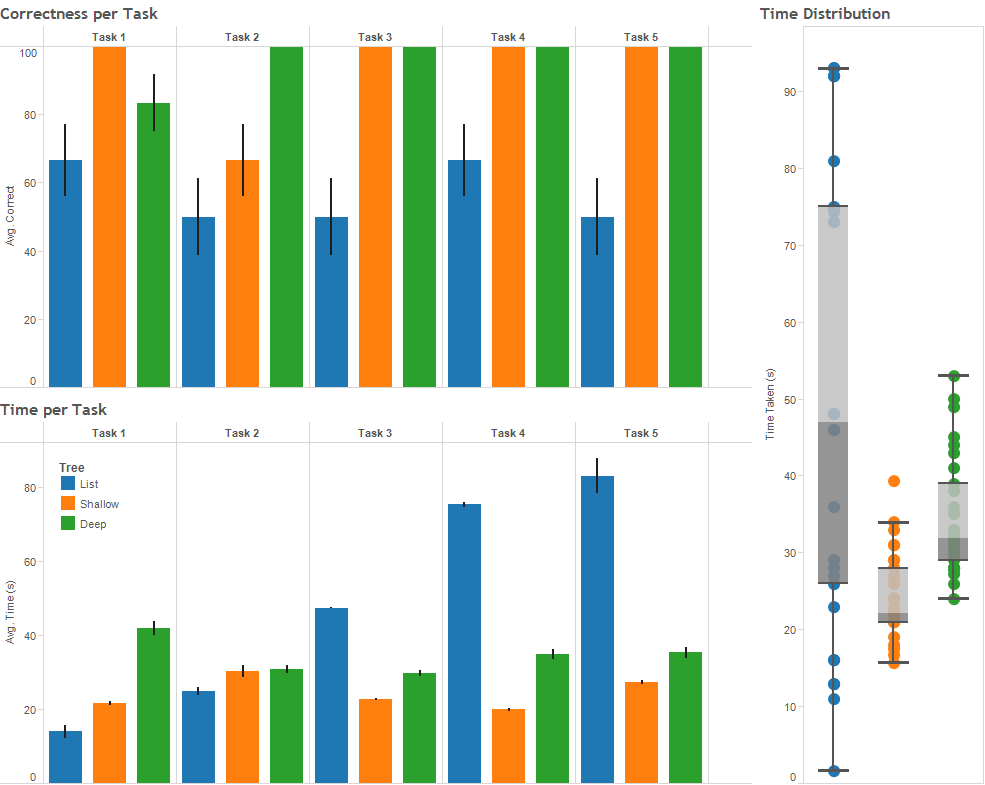
\includegraphics[width=0.9\columnwidth]{fig_CorrectnessAndTime}
    \caption{Correctness and time taken}
    \label{fig: Figure3}
\end{figure}

The correctness corresponding to each task for all design structures is depicted in Figure 3. It is clear that the hierarchical structures outperformed the linear list. Performance using the list remained poor throughout the experiment, whereas the correctness for participants using the hierarchical structures increased, as evidenced by the fact that no user incorrectly selected an item in the last three tasks. Possible explanations of these effects are discussed in more detail in the \textit{Analysis} section.

The time required to complete a task is equivalent to the amount of time a caller would spend on an IVR system. Lowering this time increases usability. The distribution of times taken by participants is shown in Figure 3. The box plots for each design structure are constructed using 30 data points, as six participants were tested for each design structure, and all users completed five tasks for the structure they were assigned. The average time taken across all tasks using the linear list structure was 48.9 seconds, the average time taken for the shallow hierarchy was 24.3 seconds, and the average time for the deep hierarchy was 34.5 seconds.

As can be seen in Figure 3, the distribution of times was largest for the list structure, where the time per task ranged from 1.7 to 93 seconds. This is because in the best case an item could be selected almost immediately, whereas in the worst case a user would have to listen to almost all 40 items before making a selection. The shallow hierarchy took the least average time, and had a range of 15.7 to 39.3 seconds. The deep hierarchy performed relatively worse than shallow hierarchy and the values were distributed from 24 to 53 seconds. 

\begin{figure}[!h]
    \centering
    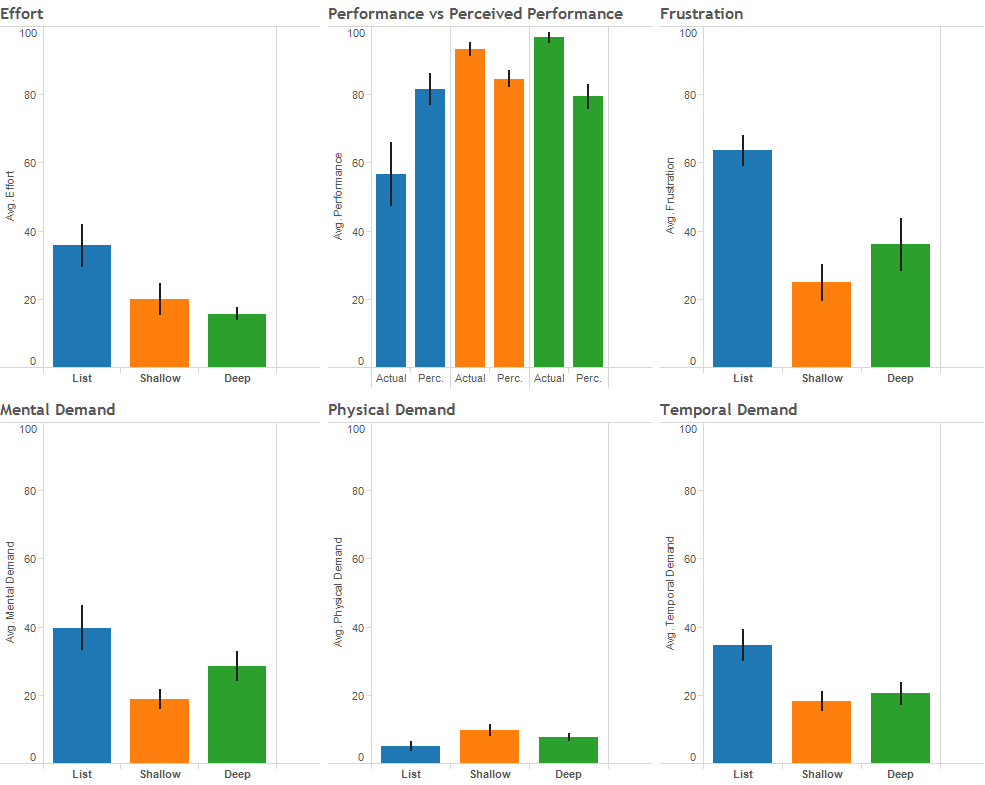
\includegraphics[width=0.9\columnwidth]{fig_nasaSummary}
    \caption{User self assessment of workload during the experiment}
    \label{fig: Figure4}
\end{figure}

After completing the experiment, user feedback was collected using the NASA TLX Survey \cite{NASA1986}. Subjects were asked to provide subjective measures on a scale of 0 to 100 to mark their effort, frustration, and perceived performance during the task. They were also asked to provide the degree of mental, physical, and temporal demand while completing the task. The results of this self-reported feedback are displayed in Figure 4.


On average, users found that list structure required the most effort. They also found it most mentally and temporally demanding, as well as the most frustrating. The shallow and deep hierarchies were comparably less physically and temporally demanding than the list. However, the deep hierarchy was on average more mentally demanding for participants. This mirrors the findings \cite{Medhi2013a} that successful navigation of the deep hierarchy required greater abstraction and reasoning capabilities than the other structures.

Also shown in Figure 4 is perceived performance compared to actual performance. After completing the task, participants were asked to indicate how well they felt they performed on a scale of 0 to 100. Participants using the list rated themselves as high performing (average score of 81.5 out of 100). This is much higher than their actual performance score (57.7 out of 100). Users of the hierarchical structures saw the opposite effect; they rated themselves lower than they actually performed. Subjects with the shallow hierarchy claimed an average of 84.5\% correctness rate but achieved 93.3\%, while participants using the deep hierarchy claimed an average of 79.3\% correctness rate but achieved 96.7\%.

\section{Analysis and Recommendation}
This work compared three design structures to organize information in an IVR system with the aim to increase information absorption and decrease information seek time. Looking at correctness and length of call measures, it is clear that the list structure is not a good choice. The correctness rate for the tasks performed on the list structure was worse, and the participants also exhibited a wide time distribution while navigating the list. Users of the linear list structure also expended the most effort, were the most frustrated, and experienced highest mental and temporal demands. Under some circumstances, correctness might be put at a premium over usability. In these cases, one might argue that the list structure could still be the best choice for certain situations. If the IVR system was providing important information concerning a disease outbreak, for instance, it could be most important that the correct information is communicated rather than that users enjoyed using the system. The list structure also fails in this scenario, however, as users were dramatically less likely to select the correct target items using the list.

The shallow and deep hierarchies performed better than the list. Part of the high performance in the hierarchical structures may be attributed to the fact that users receive instant feedback while navigating the structure. For example, two users of the list structure did not mentally parse the call correctly. Consequently, they associated numbers with the incorrect item. These two users obtained zero success rate. For instance, if the system read \textit{"For pants, press one. For shirt, press two"}, the participants bracketed the recording incorrectly and heard it as \textit{"Press one for shirt"}. They incorrectly deciphered the grouping despite completing the demonstration task. In hierarchical structures, however, while listening to a prompt \textit{"For clothing Press one, For jewelry Press two"}, if a participant intended to press a digit for \textit{clothing} but instead heard a list of jewelry items, they would have the opportunity to realize that they made an incorrect selection. Users of the list did not have this opportunity, as their first selection was a terminal item. Indeed two users of the hierarchies selected the wrong list and returned to the previous level by pressing zero, indicating that incorrect choices can be corrected by the user in a hierarchical structure.

Additional sources of error can be attributed to disagreements with hierarchy structure, confusion over items, and frustration. During the \textit{find Pants} task, several users of the deep hierarchy expressed concern that the item could be in any of the clothing categories, as men, girls, and women all wear pants. During the \textit{find Blouse} task, two female users selected shirt. Later in the experiment, when hearing blouse as an explicit option, they remarked that they realized they had made a mistake. Finally, one user of the list structure became frustrated and simply entered a random number while performing the last task rather than listening to the list items carefully again. This accentuates the importance of designing usable IVR interfaces. 

Between the two non-list structures, the shallow hierarchy is recommended over the deep hierarchy. The two gave comparable accuracy scores. The shallow structure, however, required an average of 10 seconds less per task, and was found relatively less frustrating and less mentally demanding by users.

Although using a hierarchical structure resulted in higher accuracy and lower seek time than a linear list for forty household items, it might still be better to use list for small datasets (i.e. it contains less than 10 items). The results for time completion rate for tasks (see Figure 3) indicate that the seek time to find the information in a list is much lower than the hierarchical structures until task 2. Task 2 required people to listen to up to 9 items in a linear list.  Moreover, some users also felt confused while pressing multiple digits to provide input (e.g. a one followed by a zero to select the tenth item). The correctness in the list can be improved by recording more clear prompts. Thus, we would recommend using a linear list over hierarchical structures if the dataset has less than 10 items. Within deep and shallow hierarchies, we recommend limiting the final list of items at each leaf to less than 10.


\section{Future Work}
We will recruit visually impaired and low-literate people from India to participate in our study. We will work with a local organization in Madhya Pradesh to gain access to these marginalized communities. We will measure the recruited participants on three variables:
\begin{itemize}
\item Literacy level (low, medium/high)
\item Cognitive skills (low, medium/high)
\item Familiarity to IVR usage (limited, medium/high)
\end{itemize}

Previous research has indicated strong correlation between literacy level and cognitive skills \cite{Reis2001,Medhi2013a}. Thus, we will group participants in 4 groups on the basis of the level of cognitive skills and familiarity with IVR:

\begin{itemize}
\item People with low cognitive skills and limited IVR experience
\item People with low cognitive skills and medium/high IVR experience
\item People with medium/high cognitive skills and limited IVR experience
\item People with medium/high cognitive skills and medium/high IVR experience
\end{itemize}

The fact that some users disagreed with the choices made in the deep hierarchy highlights an issue that is not discussed in this paper: hierarchy quality. Our hierarchies were chosen from the prior work \cite{Medhi2013a,Medhi2013b} and retained for the sake of comparability. The appropriateness of the hierarchy is an important element of usability, and has been addressed in other work partly through the notion of information scent \cite{Pirolli2003}. Ideally all hierarchies used in a comparison study would pass an objective measure of quality; however, valid conclusions can still be drawn with imperfect structures. The list, for example, was outperformed by both hierarchical structures even though they may not have been optimal, suggesting that a flat list is not an appropriate IVR interface for 40 items.

An additional question is how well our conclusion to use shallow hierarchies over deep hierarchies will scale to datasets comprising more than 40 items. With very large datasets, the distinction between shallow and deep hierarchies might begin to blur. We will run experiments to measure performance of various sets of deep and shallow hierarchical structures.

\section{Conclusion}

IVR systems are a valuable information and communication tool for a large number of visually impaired and low-income, low-literate users in the developing world. Making these systems effective and user-friendly in terms of information absorption and search time are key components of their usability. Although this work has focused on educated graduate students in the developed world, it has laid the groundwork for future studies that will be executed with the target population in India.

This study is motivated by real world problems and is directly comparable to existing work. We find that, for a set of 40 items, a shallow hierarchy outperforms a linear list and a more finely detailed deep hierarchy. In order to reach populations that remain out of reach of developments in graphical user interfaces, it is important that researchers focus on problems such as these that leverage existing technologies to collect data and provide information to marginalized communities in the developing world. 

% Balancing columns in a ref list is a bit of a pain because you
% either use a hack like flushend or balance, or manually insert
% a column break.  http://www.tex.ac.uk/cgi-bin/texfaq2html?label=balance
% multicols doesn't work because we're already in two-column mode,
% and flushend isn't awesome, so I choose balance.  See this
% for more info: http://cs.brown.edu/system/software/latex/doc/balance.pdf
%
% Note that in a perfect world balance wants to be in the first
% column of the last page.
%
% If balance doesn't work for you, you can remove that and
% hard-code a column break into the bbl file right before you
% submit:
%
% http://stackoverflow.com/questions/2149854/how-to-manually-equalize-columns-
% in-an-ieee-paper-if-using-bibtex
%
% Or, just remove \balance and give up on balancing the last page.
%
\balance

\bibliographystyle{acm-sigchi}
\bibliography{library}
\end{document}
